\chapter{Development}
This chapter describes the necessary steps to achieve this work's objectives. Given the complexity of the Hadoop framework, this work was divided in four stages, this decision was taken aiming mainly on understanding the context in which the scheduler will have to adapt and how it will be achieved, leaving the implementation stage to the end when every other prerequisite for the code insertion on Hadoop is already concluded. The first stage had the focus on installation and configuration of versions 1.0.4 and 2.0.3 (YARN), in order to enlarge the knowledge about the environment requirements necessary to utilize the framework. The second stage had the objective of installing and preparing the environment to compile the code, since the objective is changing the Apache Hadoop behavior and that is done by making changes in the code. The third stage was destined to the Hadoop's architecture study, through the standard Hadoop schedulers and related classes code and the Resource Manager and Node Manager state machines. Finally the fourth stage is the development and testing stage.

%-------------------------------------------------------------------

\section{Understanding Apache Hadoop internals}
\label{sec:grafo}
Aiming to insert context-awareness on a scheduler, it is necessary that the architecture of Apache Hadoop is comprehended. This stage of the project had the objective to identify the dependencies between the classes, besides which classes would be necessary to implement and how would this implementation take place.

Since a working scheduler requires many abstract classes and interfaces to be implemented, it is a good practice to know the origins of these components and how they influence the final class. Also, through the architecture study  it is possible to identify the resources supported by the framework, making it possible to decide the scheduling strategies.

Two methods were used in order to study the architecture. The first method consisted on source code study, while the second method was a study of the state machines that dictate the functioning of Resource Manager. This stage was planned aiming  the identification of all components inside a scheduler, since the implemented interfaces and abstract classes to the scheduling criteria and how these are applied on available schedulers.

\subsection{Code structure and class diagrams}

Given the framework's complexity, it was decided to use an IDE on the execution of the first method, in this case the chosen IDE was IntelliJ IDEA \cite{IDEA}. Once the study was finished, it was possible to generate a series of class diagrams. The generated diagrams were used in conjunction with HortonWorks  Diagram in order to make the understanding of the whole YARN framework easier.

The first diagrams used in this step were the ResourceManager and NodeManager component diagrams, which provided a better high level understanding of the components that compose the ResourceManager and NodeManager.

The figure \ref{fig:RMHorton} illustrates the high level view of the ResourceManager. It is possible to note many modules which doesn't matter to the context of this work, such as: Security, DelegationTokenRenewer, among others. Even so, the notion this figure passes has a high value to the understanding.

\begin{figure}[hbtn]
   \renewcommand{\figurename}{Figure}
   \centering
   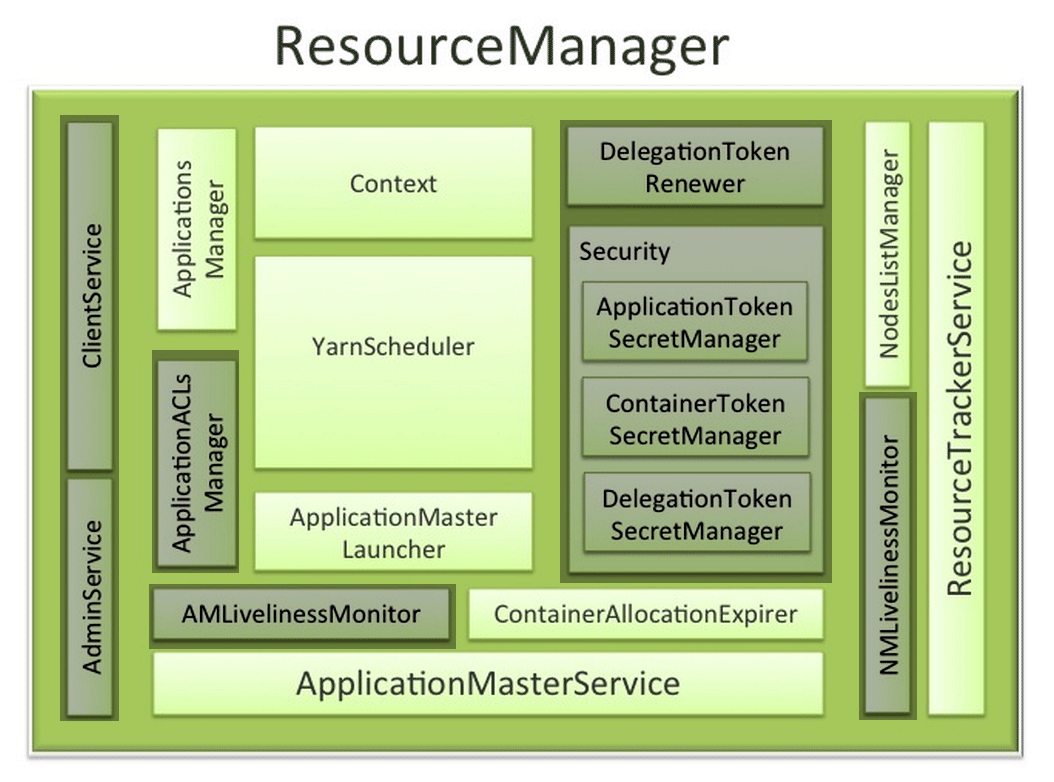
\includegraphics[width=15cm]{figuras/Figura14-RMHorton.png}
   \caption{ResourceManager Component Diagram \cite{HortonRM}}
   \label{fig:RMHorton}
\end{figure}

The ResourceManager is the master that arbitrates all the available cluster resources and thus helps manage the distributed applications running on the YARN system. It works together with the per-node NodeManagers (NMs) and the per-application ApplicationMasters (AMs) \cite{HortonRM}.

Except the scheduler itself, there are other components of fundamental importance to the scheduling process. Like the ApplicationsManager, which manages all the submitted applications. The ApplicationsManager component not only has a list of submitted applications, but also has information about all the completed applications and is able to provide this through either web UI or command line.

Another important component is the ApplicationMasterLauncher, that will be responsible to create the application specific ApplicationMaster, everytime an application is submitted. Another task left to the ApplicationMasterLauncher component is the deletion of ApplicationMaster when the application has finished, either normally of forcefully.

The ApplicationMaster itself is a concept that makes YARN completely different than the previous Hadoop versions. It is a key component on MapReduce tasks execution because it has one instance for every application being executed, making the ApplicationMaster the component responsible for the execution and monitoring of the containers and their resource consumption. Therefore, it has to communicate with the ResourceManager in order to ask and report the status and progress of its monitored containers.

It is through ApplicationMaster that YARN can achieve better scalability, since it takes some of the processing usually delegated to the Scheduler and ResourceManager components. One of the key tasks that was transferred to the ApplicationMaster is the fault tolerance. It is the ApplicationMaster that will decide when and/or if a speculative task is necessary and beneficial. Thanks to this shift in the responsibilities and the ApplicationMaster being a per-application manager, the cluster scaling potential is improved through the removal of a possible bottleneck. 

Another crucial component to the present work is the ResourceTrackerService, that is responsible for the communication with the NodeManagers. This is the component that answers to the RPC calls, whenever a node wants to register with the RM, send a heartbeat, or many other tasks, this is the component that will be used. The node capacity is also passed on the registration of a node with the RM, this process of registration will store the node's information in the NodesListManager. The second component is a collection of all the nodes, both the valid and the decomissioned ones.

Finally, the Scheduler follows the same pattern as regular scheduler, comparing requests, availabilities and then granting the resources based on some heuristic. However, most Hadoop schedulers use queues in order to help the task of managing the users and application submitted.

The other high level view that interests this work is the NodeManager. Just as the ResourceManager counterpart, even having some irrelevant modules presented in the figure \ref{fig:NMHorton}, it facilitates the understanding of the service in a high level. Having a high level understanding is necessary in order to understand how the two services will interact.

\begin{figure}[hbtn]
   \renewcommand{\figurename}{Figure}
   \centering
   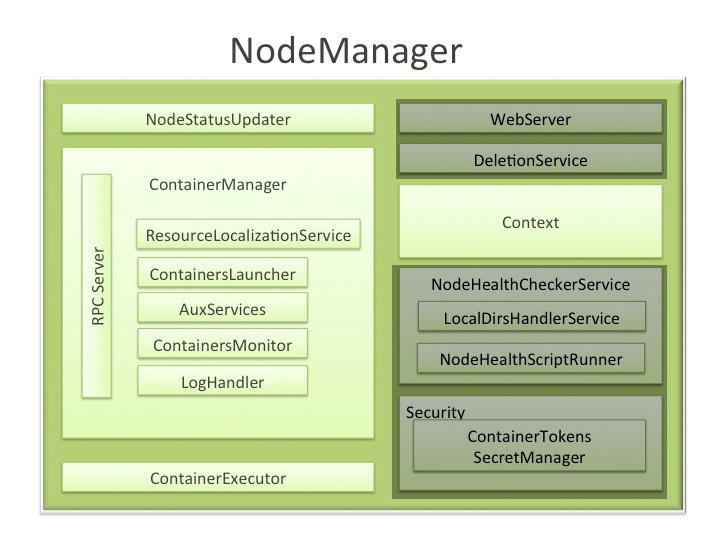
\includegraphics[width=15cm]{figuras/Figura15-NMHorton.png}
   \caption{NodeManager Component Diagram \cite{HortonNM}}
   \label{fig:NMHorton}
\end{figure}

Each slave will have a NodeManager instance running, which is the local manager. This service main responsibility is keeping his information updated on the ResourceManager, but it has other attributions like managing the containers, monitoring the resource usage, monitoring node health, among others.

One key component is the NodeStatusUpdater, which will be responsible for the registration with the ResourceManager, it is through registration that the ResourceManager will be informed about the resources of a given node, making this component vital for the success of the approach in this work. Also, after the initial registration this component is expected to maintain the communication with the ResourceManager in order to provide updates on containers launched, running or completed.

The largest component in the figure, the ContainerManager is as important as its size implies. With help from its sub-components, the ContainerManager has the hard but extremely necessary task of monitoring containers and informing whatever component needs this information. There are several ContainerManager sub-components, they are: RPC server, ResourceLocalizationService, ContainersLauncher, AuxServices, ContainersMonitor and LogHandler. Some like the ResourceLocalizationService is of vital importance to the MapReduce tasks, as it downloads the files that will be used on the tasks' execution, but won't interfere in this work's context.

The next diagram used to better understand the architecture was the scheduler components class diagram, which provided a helped to view classes related to the scheduling process. The Scheduler Components Class Diagram can be visualized in the figure \ref{fig:SchedCD}.

\begin{figure}[hbtn]
   \renewcommand{\figurename}{Figure}
   \centering
   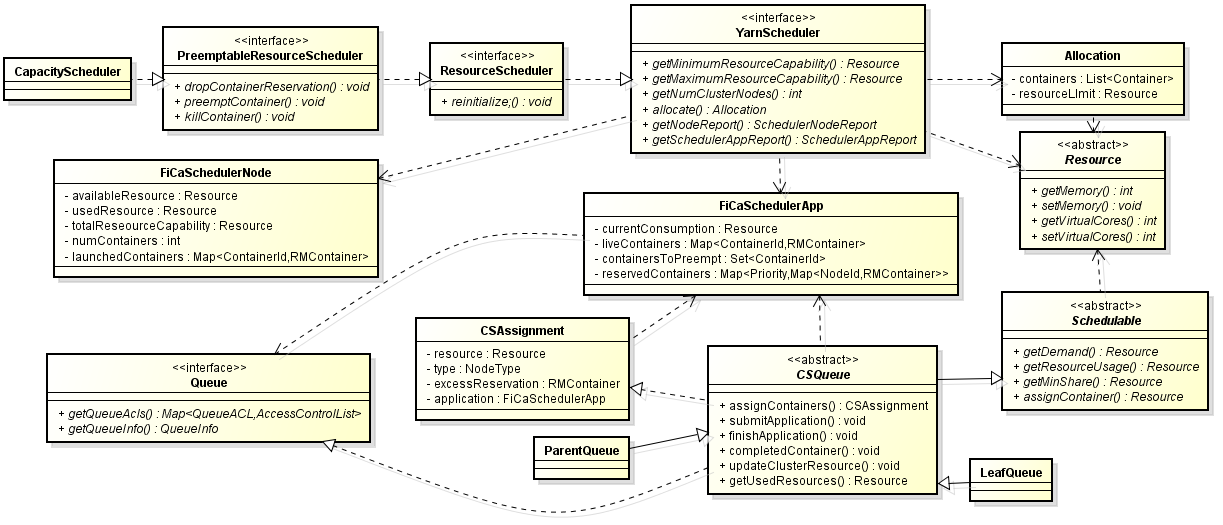
\includegraphics[width=15cm]{figuras/Figura01-ClassDiagram.png}
   \caption{Class Diagram with the main CapacityScheduler classes}
   \label{fig:SchedCD}
\end{figure}

Following is a description of the main components that compose the CapacityScheduler:
\begin{itemize}
	\item Schedulable: an abstract class that represents an entity capable of launching either a job or a queue, it offers a simple interface whereby the algorithms can be applied either inside a queue as well as several queues.
	\item Queue: an interface that enables the basic control of all the queues in the scheduler. Possessing methods to allow reading of the queue info, and also queue management.
	\item PreemtableResourceScheduler: another interface that allows the preemption of resources, through the scheduler.
	\item Resource: an abstract class responsible for modelling the resources capable of being use, which at this moment are only memory and core count.
	\item FiCaSchedulerNode and FiCaSchedulerApp: representations of the node and application, provides vital information about the structures. Uses a lot of the components present on the next Class Diagram.
\end{itemize}

Another key class diagram to the context of this work was the diagram that would represent three very important components, the RMContainer, RMNode and RMApp/RMAppAttempt. All of these components represents fundamental parts on understanding how this work has impacted the scheduling. RMContainer is the name given to the reservations of resources, making it also responsible for the task execution. RMNode is the representation of a whole NodeManager to the scheduler, and is through it that the scheduler will get access to the NodeManager real resource capacity. RMApp and RMAppAttempt represents the applications sent to the scheduler. This diagram is represented in the figure \ref{fig:RMComponents}.

\begin{figure}[hbtn]
   \renewcommand{\figurename}{Figure}
   \centering
   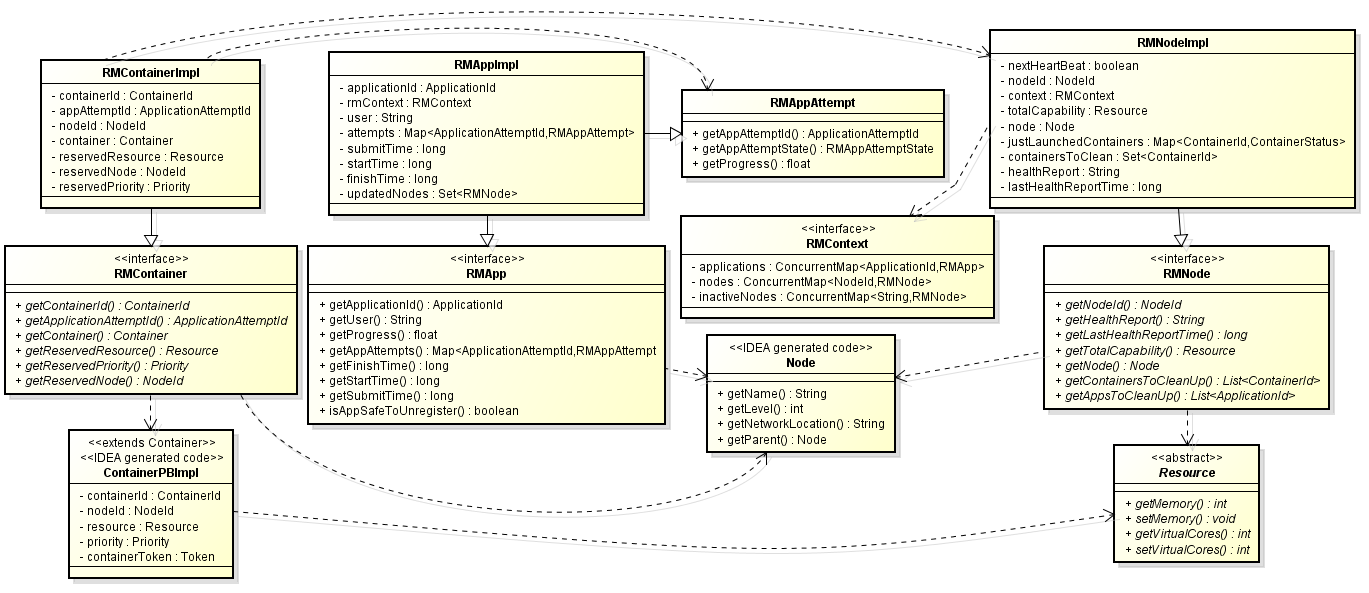
\includegraphics[width=15cm]{figuras/Figura13-RMComponents.png}
   \caption{Class Diagram with the main RM components}
   \label{fig:RMComponents}
\end{figure}

\subsection{State machines}

The second method was executed through an option offered by the Maven tool, in which it is possible to generate graphs that represents the Resource Manager and Node Manager state machines. Through analysis of the graphs it is possible to identify the life cycle of some key components, such as RMContainers, RMNodes and RMApplications. 

The importance of RMContainers, RMNodes and RMApplications may be overlooked until further analysis of source code and state machines at the same time. It is not a coincidence that all the components have a RM, referencing ResourceManager, in their names. In a brief explanation, RMNodes have all resource and other static information concerning a given NodeManager. RMContainers are the structures that represent the reservation of resources and also responsible for the processing. Finally, the RMApplication is the component that provides ResourceManager a way to access application status, reports and updates. All state machines and a more thorough explanation can be found on \autoref{chap:ApendA}.

%-------------------------------------------------------------------

\section{Understanding Hadoop allocation pattern}
\label{sec:alloc}
In order to improve Hadoop resource utilization and change the resource allocation behavior, it was necessary to understand how the allocation is made. That implies knowing and understanding the whole process of requisition and grant of resources, which is essentially the scheduling. After the experiments made with the objective of understanding this process, it was possible to identify which parameters influenced and how much impact would these parameters have once they were changed.

Once a quick research on official documentation and the parameters which can be set on XML files was made, it was found that there are five parameters that influence the allocation pattern for each resource. These parameters can be roughly divided into three classes: application request, cluster configuration towards containers and cluster configuration towards ApplicationMaster (AM). All of these parameters have default values in case the application did not set a request value or the cluster administrator did not set them properly on configuration files.

The application request parameters are set through the JobConf class when the user is coding his MapReduce job. If the parameters are not set at this time, the cluster will use the properties \textit{mapreduce.map.memory.mb} and \textit{mapreduce.reduce.memory.mb} either at the \textit{mapred-site.xml} or \textit{mapred-default.xml}, following default Hadoop behavior towards settings in the xml files. The default behavior is: if the properties are set in any \textit{*-site.xml} file that's the value they will assume, otherwise the values will be taken from \textit{*-default.xml} file.
The default value for properties \textit{mapreduce.map.memory.mb} and \textit{mapreduce.reduce.memory.mb} is 1024.

The cluster configuration towards containers is composed by four parameters, these parameters express the floor and ceiling of valid allocations. The floor limit parameters receive their values from the properties \textit{yarn.scheduler.minimum-allocation-mb} related to the memory and \textit{yarn.scheduler.minimum-allocation-vcores} related to the cores, while the ceiling limit parameters receive their values from properties \textit{yarn.scheduler.maximum-allocation-mb} and \textit{yarn.scheduler.maximum-allocation-vcores}. All properties will follow the default Hadoop behavior towards settings in XML files. These four parameters are related to two variables in the source code, which are named \textit{minimumAllocation} and \textit{maximumAllocation}, which represents the floor and ceiling limit respectively. 
The default value for \textit{yarn.scheduler.minimum-allocation-mb} is 1024 and the default value for  \textit{yarn.scheduler.minimum-allocation-vcores} is 1. The default values concerning the ceiling properties is 8192 for \textit{yarn.scheduler.maximum-allocation-mb} and 32 for \textit{yarn.scheduler.maximum-allocation-vcores}.

The only parameter left is the AM request, this request will be the same for every application submitted to the cluster and cannot be configured through JobConf. This parameter will receive it's value from properties \textit{yarn.app.mapreduce.am.resource.mb} related to the memory and \textit{yarn.app.mapreduce.am.resource.cpu-vcores} related to the cores, also following the default Hadoop behavior. The default value of the parameter \textit{yarn.app.mapreduce.am.resource.mb} is 1536, and, the default value of the parameter \textit{yarn.app.mapreduce.am.resource.cpu-vcores} is 1.

\subsection{Experiment}
In order to understand how the allocation process is made an experiment was performed. The experiment was made aiming to understand how the RM allocates memory for applications given requisition and minimum/maximum parameters changes. It consisted in altering some of the parameters and analysing the resultant behavior. As the AM request is the same across the cluster, it was excluded from the experiment. The reason being that different applications would have the same amount requested by the AM and it's behavior follows the same pattern as the other requests, which are easier to manipulate.

\subsubsection{Employed methods, procedures and scenarios}
The experiment was performed in a cluster deployed on Grid'5000 environment. The cluster had five nodes, one master and four slaves, each node having the following configuration: 2 CPUs AMD@1.7GHz, 12 cores/CPU and 47GB RAM. All nodes were running an Ubuntu-x64-1204 standard image, having Sun JDK 1.7 installed. The Hadoop distribution was the 2.2.0 YARN version.

The procedure chosen as data acquisition method was the Hadoop Log System. The reason for such a choice was that Hadoop Log System is, by default, enabled in the INFO level and using the INFO level would be possible to insert small entries and extract useful information in real time.

Following there is a brief description of the four scenarios used in the experiment:

\begin{itemize}
	\item \textbf{Default scenario}: no parameter was changed.
	\item \textbf{Requisition higher than maximum}: the application requested an amount of memory higher than the cluster maximum allocation parameter. The changed value was the maximum allocation memory. The minimum was also changed for consistency reasons.
	\item \textbf{Requisition smaller than minimum}: the application requested an amount of memory smaller than the cluster minimum allocation parameter. The changed value was the minimum allocation memory.
	\item \textbf{Requisition inside range}: the application requested an amount of memory inside the cluster valid range. The changed values were the minimum allocation memory and requisition from both map and reduce.
\end{itemize}

\subsubsection{Results and interpretation}

The results from the scenarios can be analysed on the figure \ref{fig:memory allocation}.

\begin{table}
	\renewcommand{\figurename}{Table}
	\centering
	\begin{tabular}{|l|c|c|c|c|}
		\hline 
		Parameters & Default & Higher & Smaller & Inside\\ 
		\hline 
		Map Memory Requisition (MB) & 1024 & 1024 & 1024 & 3456\\ 
		\hline 
		Reduce Memory Requisition (MB) & 1024 & 1024 & 1024 & 3712\\ 
		\hline 
		Minimum Memory (MB) & 1024 & 512 & 2048 & 512\\ 
		\hline 
		Maximum Memory (MB) & 8192 & 768 & 8192 & 8192\\ 
		\hline 
		Map Memory Allocation (MB) & 1024 & ERROR & 2048 & 3584\\
		\hline
		Reduce Memory Allocation (MB) & 1024 & ERROR & 2048 & 4096\\ 
		\hline 		
	\end{tabular}
	\caption{RM memory allocation pattern experiment results}
	\label{tab:memory allocation}
\end{table}

\begin{figure}[!hbtn]
   \centering
   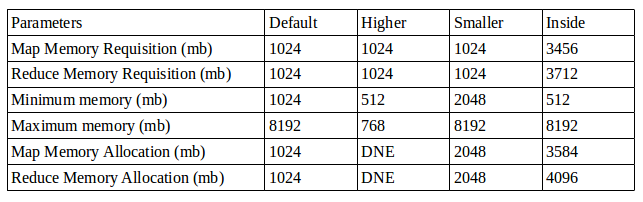
\includegraphics[width=15cm]{figuras/Figura09-allocation.png}

\end{figure}

Because of the experiment, it was possible to detect that Hadoop allocation pattern differs a bit from usual. Unlike usual pattern in which if a request is inside the minimum and maximum range, the amount granted is equal to the request, the requests on Hadoop will pass through a small set of calculations in order to determine how much memory will be granted.

The figure \ref{fig:fluxoAllocation} portraits the  flow of operations executed by the Hadoop in order to determine the granted resources.

\begin{figure}[!hbtn]
   \renewcommand{\figurename}{Figure}
   \centering
   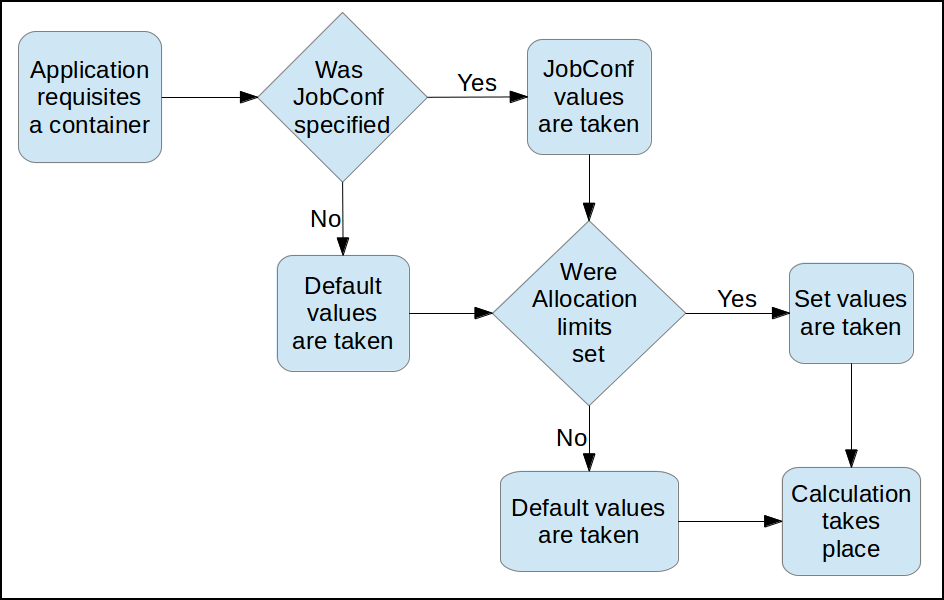
\includegraphics[width=15cm]{figuras/Figura18-allocflow.png}
   \caption{Flow of operations for resource granting}
   \label{fig:fluxoAllocation}
\end{figure}

The default scenario just demonstrates how Hadoop allocation will behave in case there are no interventions.

The second scenario shows what happens if the application requests a value higher than the maximum. The output is an error message and the job execution is aborted.

The third scenario shows what happens if the application requests a value smaller than the minimum. The cluster grants the minimum allowed.

The fourth scenario shows a case in which the requests are inside the valid range but although the requests were similar, the resources granted were different. This scenario is the one that makes it possible to fully comprehend the allocation process. Since the second and third scenarios provided evidence that a request can't be higher than the maximum and that at least the minimum allocation will be given, it is possible to infer that the allocation will always start with the minimum allocation value. In the case the minimum allocation is not enough to satisfy the request, the value which will be granted is always incremented by the minimum allocation until it matches one of the following cases: the value is equal to the request, the value is higher than the request and lower than the maximum allocation or the value exceeds maximum allocation. Concerning the scenario, it is the second case that occurs.

The figure \ref{fig:fluxoAllocation2} is provided along with extensive explanation to facilitate the understanding of the whole calculation process. 

\begin{figure}[!hbtn]
   \renewcommand{\figurename}{Figure}
   \centering
   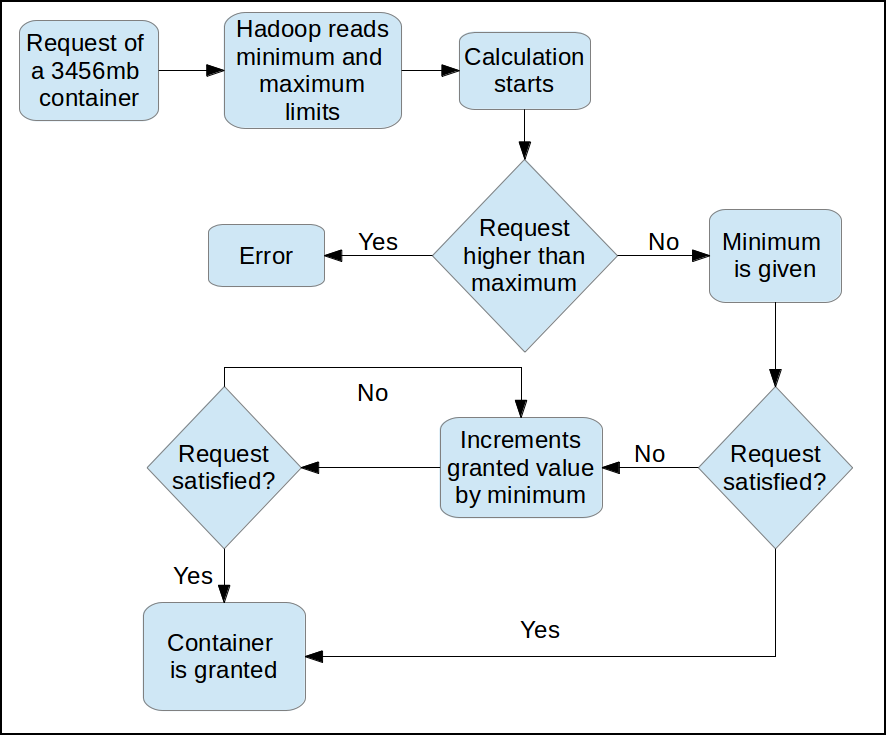
\includegraphics[width=15cm]{figuras/Figura19-allocflow2.png}
   \caption{Flow of operations for resource granting}
   \label{fig:fluxoAllocation2}
\end{figure}

The step by step calculation on scenario four will be demonstrated. Assuming M is the memory granted, or in the process of calculation, for the map request and R for the reduce. The calculation happens as follows:

Firstly the M and R are set to the minimum memory allocation property, which is 512. Since 512 does not satisfy any of the requests the M and R values are then incremented by the minimum memory allocation, assuming the value of 1024. As 1024 still smaller than both requisitions, they are again incremented by 512 and the process goes on as following:

M: 512, 1024, 1536, 2048, 2560, 3072, 3584.

R: 512, 1024, 1536, 2048, 2560, 3072, 3584, 4096.

Note that in both cases the value granted was the smallest multiple of minimum memory allocation (512) greater than or equal to the request (3456 and 3712).

%-------------------------------------------------------------------

\section{Context-aware scheduling}
Knowing that the scheduling task is closely related to the resources availability and, therefore, having a wrong information could ruin the performance of the algorithm, an opportunity for improvement was seen. After a quick study on the default schedulers, it was clear that CapacityScheduler already had the whole structure to support a better scheduling, as stated in the section \ref{sec:Hadoop Schedulers}. The flaw on CapacityScheduler wasn't really a scheduling flaw, but actually a wrong information received by the NodeManagers.

As stated numerous times in previous sections, Hadoop configuration is heavily dependent in XML files. While providing an easy way to configure a real cluster, sometimes it acts more as an obstacle than as a facilitator, the reason being that if one wants to change a parameter the whole service will have to be restarted. One huge restriction implied by XML files, is regarding the nodes capacity. In case one doesn't want to use Hadoop default configurations for node capacity, every node will have to have it's XML files edited. In a large heterogeneous cluster, modifying one file in each node will certainly be time consuming since each node will have a different configuration. 

One possible solution to this case, is to overwrite the value gotten from XML file on the code. At first glance this brings in more problems than solutions, because the administrator would have to chose a certain hard coded value that would fit best as an average among all nodes. However, as one looks closer into the proposal, there is an option that, although involving more coding, would solve this problem. 

It is clear that this solution requires the application to detect some context of the environment. The context, in this case, being the real information about node capacity. With this context at hands, it is a reasonable choice to make the scheduler context-aware. Therefore, improving the scheduling performance. As the section \ref{sec:ctx} implies, being context-aware requires the application to detect and adapt to changes in environment.

Regarding the detection of the node capacity, the chosen option was to integrate a collector into Hadoop, meaning that every node would be able to access it's true capacity. Thus, preventing the hard coding that was suggested.

Regarding the changes made once the context information was detected, the approach adopted was to scale the allocation limits together with the total cluster resource availability. This scaling meant that the containers would have more memory and cores at their disposal and, therefore, speculative task would hardly have to be launched. Also, by adapting to the cluster real resource, no resource would be wasted or left inactive while the scheduler is making tasks wait due to wrong information being received. Thus improving the cluster utilization.

\subsection{Collector description}
The collector of choice was PER-MARE's collector \cite{Collector}. This collector uses a standard java package in order to access the real node capacity, therefore, no additional libraries would be necessary.
 
Only four files were necessary, an interface, an abstract class and two classes. Due to it's design, it would be easy to integrate new collectors and improve the resources available for the scheduling process, providing data about the CPU load or disk usage for example.

The base of the collector is the interface Collector, which has two access methods and the collect method. 

The abstract class, called AbstractOSCollector, implements the interface and has some access methods of its own. The great usability comes from the usage of OperatingSystemMXBean, a public java interface that is used to access the operating system informations on which the Java virtual machine is running \cite{MXBean}.

The collector classes, called PhysicalMemoryColletor and TotalProcessorsCollector extends the AbstractOSCollector and have only constructor and collector method implemented.
%TODO trechos de c´odigo no appendix?

\subsection{Collector integration with Hadoop}
The collector would have to be placed on NodeManager (NM), since this is the service responsible for processing tasks. The collected capacity is then sent to the ResourceManager (RM) in the moment that each NM is registering with the RM. It is possible to view the whole process of data acquisition until CapacityScheduler add the node in the figure \ref{fig:collectorflow}.

\begin{figure}[!hbtn]
   \renewcommand{\figurename}{Figure}
   \centering
   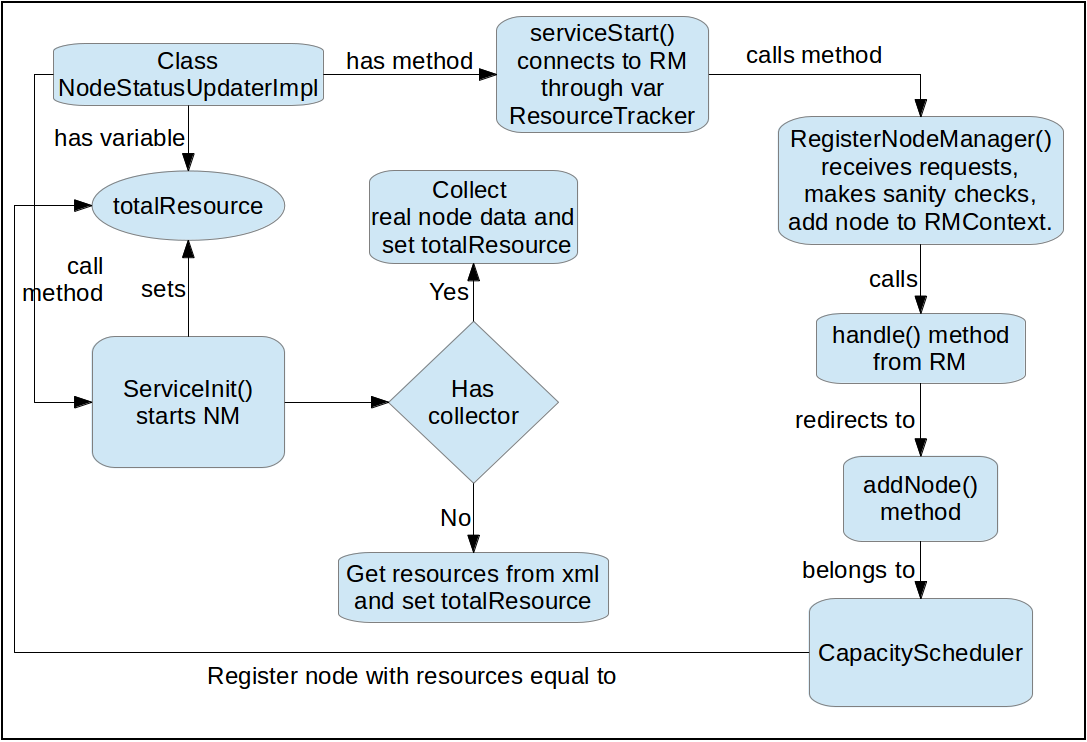
\includegraphics[width=15cm]{figuras/Figura20-collectorfig.png}
   \caption{Flow of operations for resource granting}
   \label{fig:collectorflow}
\end{figure}

After the collector integration, changing the scheduling behavior was possible due to the now available information about the real resources of a given node. Further information about the results gotten from the collector integration and modified scheduling can be found at the chapter \ref{chap:Experiments and Results}.